\section*{Mise en place}
\addcontentsline{toc}{section}{Mise en place}
\begin{figure}%
    \subfloat[\centering Le plateau central]{{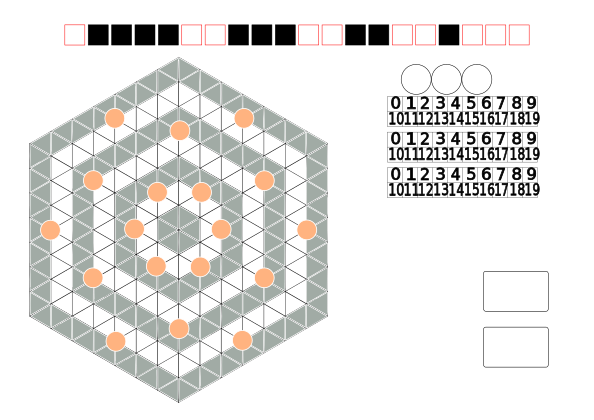
\includegraphics[scale=0.35]{regle/plateau} }}%
    \qquad
    \subfloat[\centering Le plateau de chaque joueur]{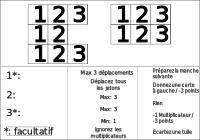
\includegraphics[scale=0.4]{regle/plateauJoueur}}%
    \caption{Les plateaux}%
    \label{fig:plateaux}%
\end{figure}
\FloatBarrier
    
Pour mettre en place le jeu, procédez ainsi:
\begin{itemize}
\item Mélangez les 15 \jetonsMeteo, et placez en 10 sur la piste de météo, aux emplacement prévu à cet effet ( \includegraphics[scale=0.35]{../ToolBox/Images/numeros/numeros_bleu1})
\item Mélangez les trois \marqueursObstacles, et placez-en un sur chaque emplacement ( \includegraphics[scale=0.35]{../ToolBox/Images/numeros/numeros_vert1})
\item Mélanger tous les \jetonsObstacles, et placez les sur les emplacement prévu, avec la face correspondante visible ( \includegraphics[scale=0.35]{../ToolBox/Images/numeros/numeros_vert2}). Ainsi, vous devez avoir un jeton de chaque couleur sur chaque niveau, avec:
\begin{itemize}
\item[*] Les \textit{rochers} à l'extérieur
\item[*] les \textit{1} sur le niveau intermédiaire
\item[*] les \textit{troncs} sur le niveau intérieur
\end{itemize}
\item Placez les randonneurs sur les six portions de chemins les plus au centre (\includegraphics[scale=0.35]{../ToolBox/Images/numeros/numeros_vert3})
\item Mélangez toutes les cartes, distribuez-en 3 à chaque joueur, et placez la pioche, \textbf{randonneur vers le haut}, sur l'emplacement prévu (\includegraphics[scale=0.35]{../ToolBox/Images/numeros/numeros_bleu2})
\end{itemize}
\FloatBarrier

Une fois le plateau central mis en place, choisissez un esprit que vous incarnerez (
\includegraphics[scale=0.02]{jetonsJoueurs/eau}, 
\includegraphics[scale=0.02]{jetonsJoueurs/nature}, 
\includegraphics[scale=0.02]{jetonsJoueurs/foudre}, 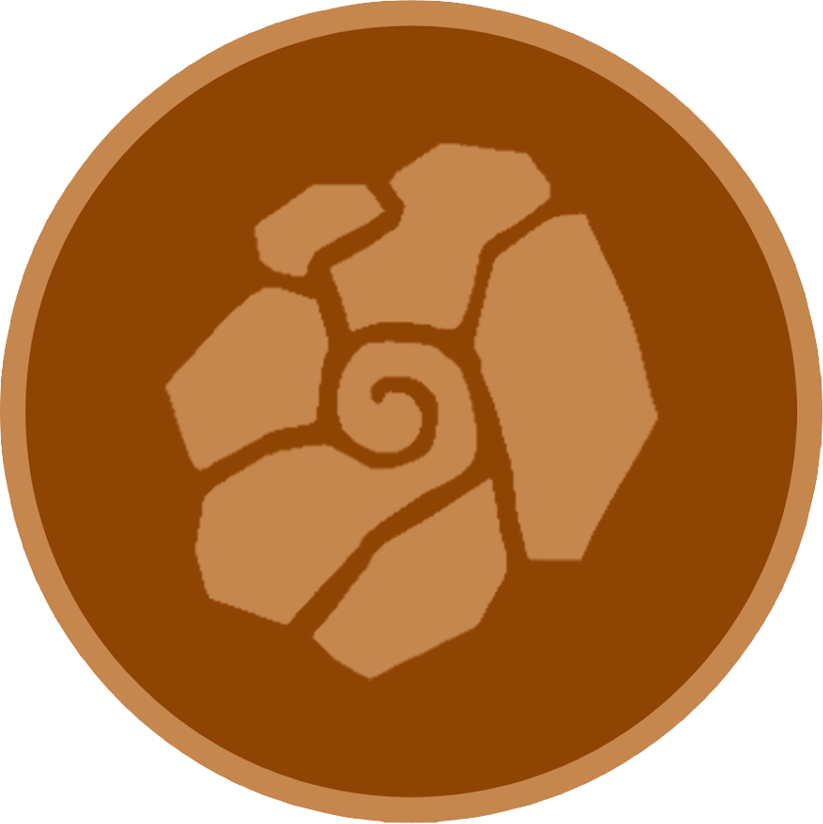
\includegraphics[scale=0.02]{jetonsJoueurs/terre}, 
\includegraphics[scale=0.02]{jetonsJoueurs/vent}). Puis:
\begin{itemize}
\item prenez le plateau correspondant
\item prenez les 9 jetons correspondants, et répartissez les ainsi:
\begin{itemize}
\item[*] Placez en un à côté de chaque piste d'obstacle (\includegraphics[scale=0.35]{../ToolBox/Images/numeros/numeros_rouge1})
\item[*] Placez en un sur la piste de score (\includegraphics[scale=0.35]{../ToolBox/Images/numeros/numeros_rouge2})
\item[*] Placez un jeton sur chaque multiplicateur, sur la case 1 (\includegraphics[scale=0.35]{../ToolBox/Images/numeros/numeros_rouge3}).
\end{itemize}
\item prenez les 6 tuiles 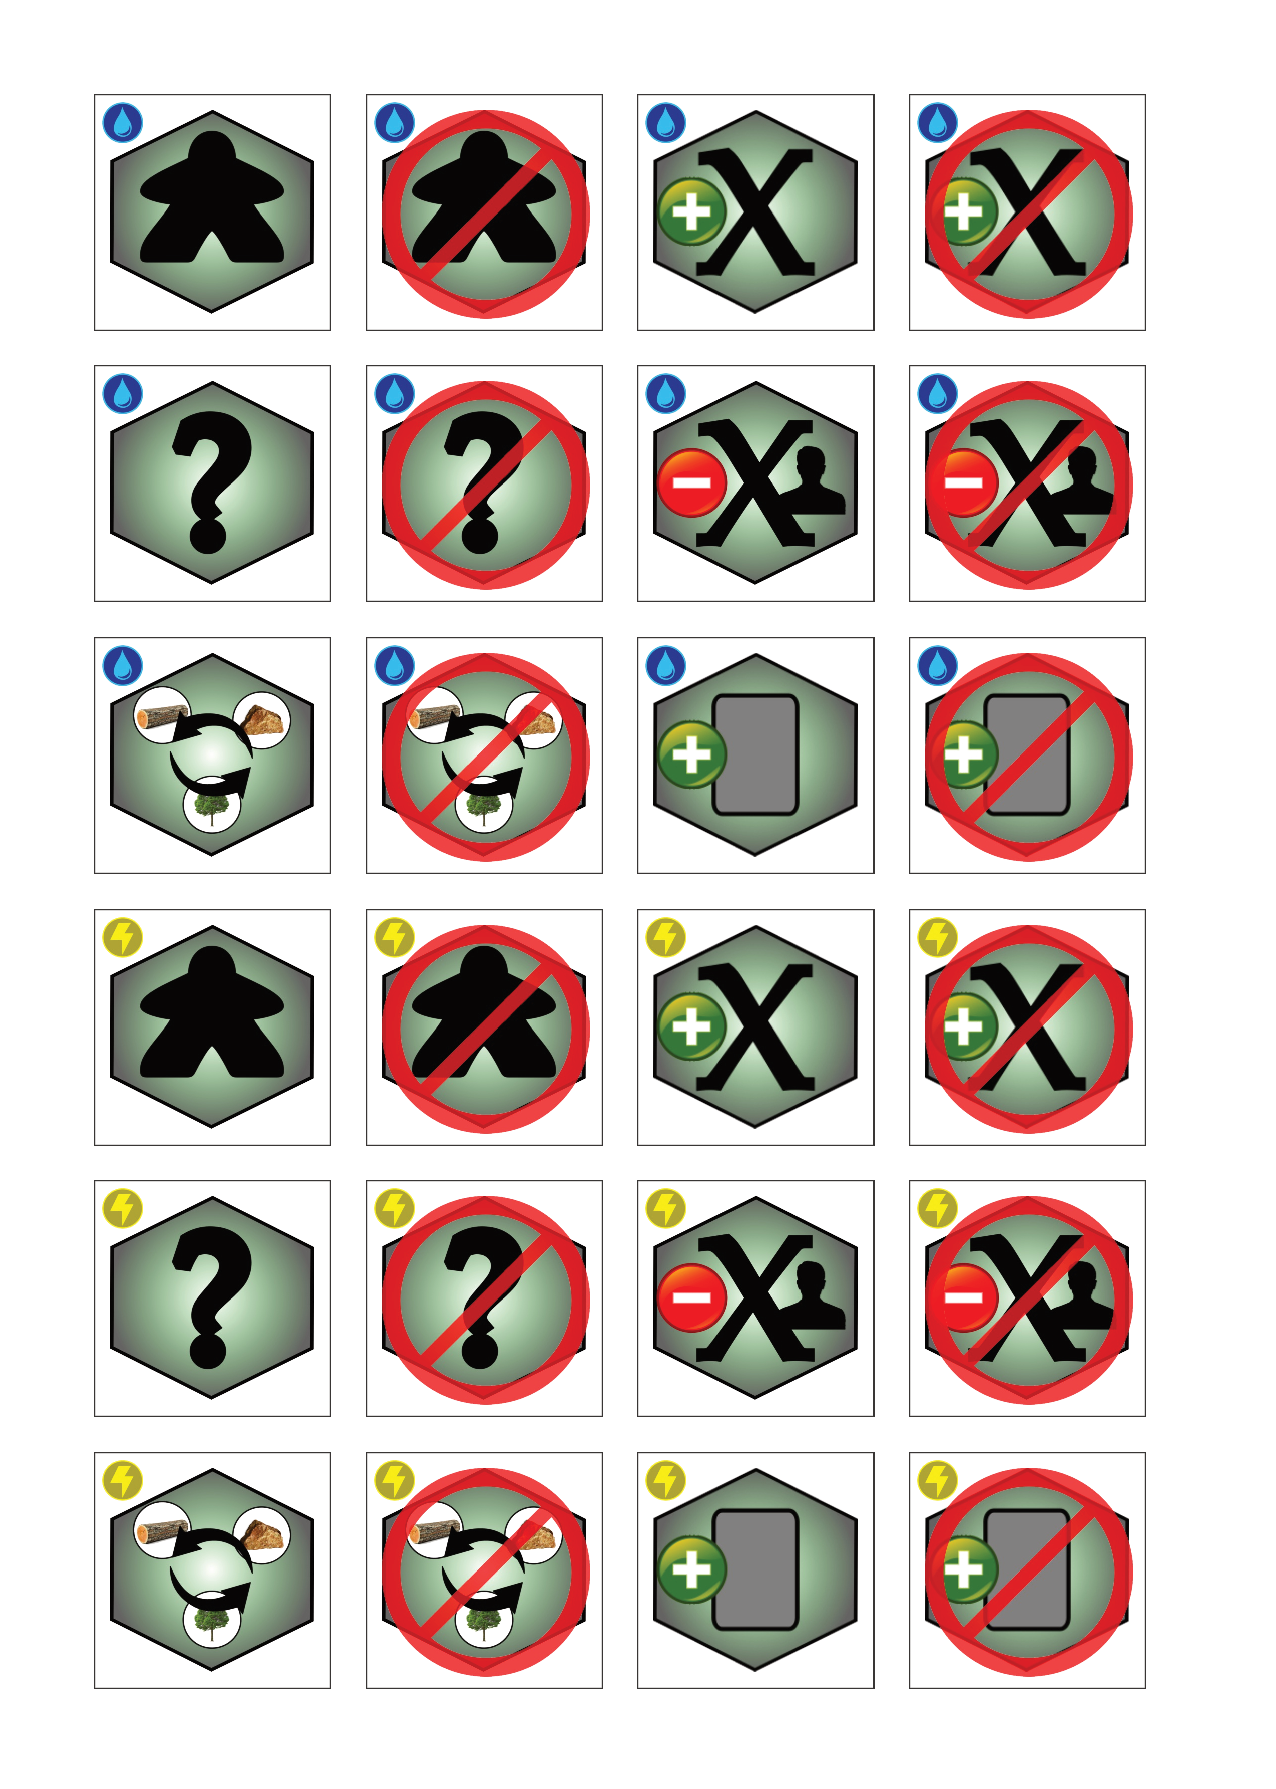
\includegraphics[scale=0.25]{regle/tuiles} de votre esprit. Placez en une sur sa face 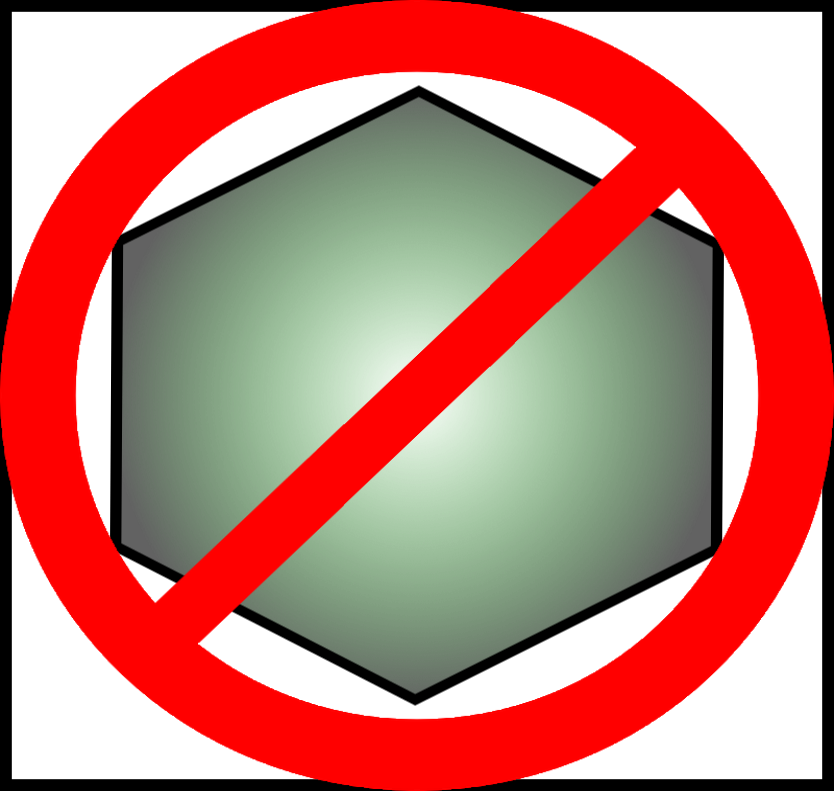
\includegraphics[scale=0.15]{icones/icones_jetonTuileBloquee} et toutes les autres sur la face 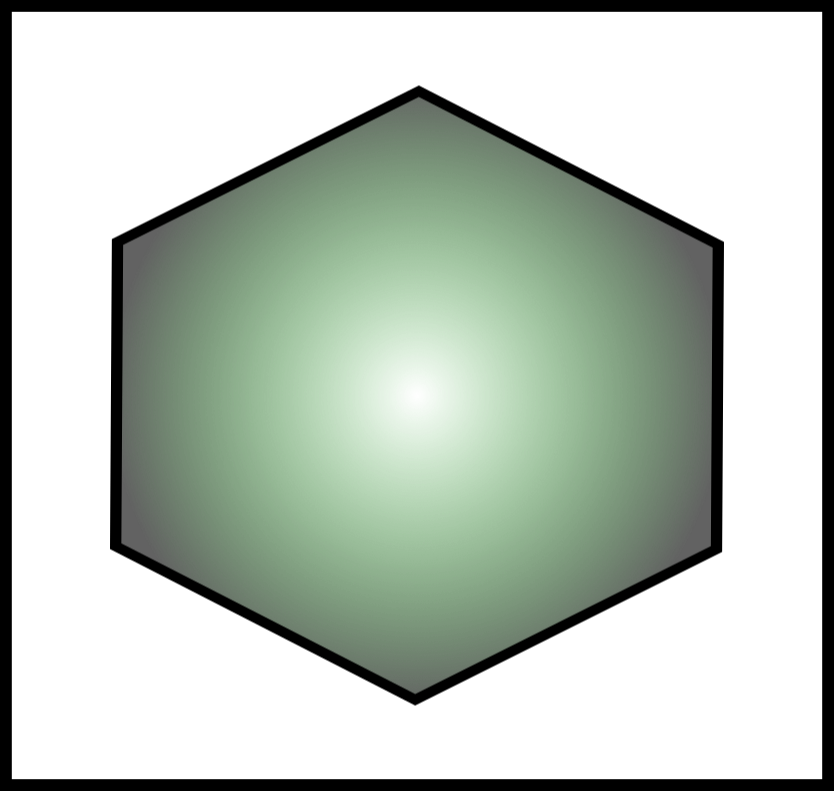
\includegraphics[scale=0.15]{icones/icones_jetonTuileActive}.
\end{itemize}
 
\subsection*{Premier joueur}
\addcontentsline{toc}{subsection}{Premier joueur}
Le premier joueur est le dernier a avoir joué au flipper. Si personne n'a joué en dernier, prenez le dernier à être allé en montagne.